\section{Design}
\label{sec-design}

\subsection{network design}


The core of the \textsf{SRPeek} system is a specially designed multi-frame SR neural network, accepting a group of $N$ images indexed $x_1^{(0)}$ to $x_N^{(0)}$ as input and generating an image with higher resolution $y$ as output. The network comprises $L$ layers, each of which implements a non-linear transformation $H_l(\cdot)$, where $l$ indexes the layer. As mentioned before, in each layer images are processed separately, with the merging layers as a revenue for communication, so that the output of each layer is correspondent to the input.  We denote the output of the $l^{th}$ layer as $x_1^{(l)}$ to $x_N^{(l)}$, which is also the input of the $(l+1)^{th}$ layer. Till now the model is not different from traditional SR models:

$$x_i^{(l)} = H_l(x_i^{(l-1)}), i=1,2,...N$$

\cl{function above cannot express merging between x1 x2 ... xN?}

Additionally, we introduce the initial images $x_i^{(0)}$ as an input for all the layers:

$$x_i^{(l)} = H_l(x_i^{(l-1)},x_i^{(0)}), i=1,2,...N$$

The last layer is exceptional, it yields a single image $y$ as output. 

Presently, in these layers nothing is done to raise the resolution of the images, so that the resolution of $x_i^{(0)}$ to $x_i^{(l-1)}$ and $y$ remains the same. To increase resolution we insert several 2$\times$ nearest upsampling layers $U$ evenly throughout the architecture between the layers:

$$x_i^{(l)} \leftarrow U(x_i^{(l)}), x_i^{(0)} \leftarrow U(x_i^{(0)}), i=1,2,...N$$

we upsample the input images $x_i^{(0)}$ simultaneously to keep the two inputs of the following layers $H_l(x_i^{(l-1)},x_i^{(0)})$ unanimous in resolution. For example, in a 4$\times$ SR network with five layers, we may insert 2 2$\times$ nearest upsampling layers behind the 2nd and 4th layer.

Inside each layer $H_l$ there are 3 convolution layers $Conv_{1l}(\cdot)$, $Conv_{2l}(\cdot)$, $Conv_{3l}(\cdot)$ and 1 merging layer $Merge_l(\cdot)$, distributed as follows:

\cl{$H(\cdot)$ or $H(\cdot,\cdot)$?}

\begin{enumerate}
\item The first input parameter of this layer, $x_i^{(l-1)}$, is passed through a convolution layer to extract features. Note that all three convolutional layers accept a single image(or its featuremaps from the last convolutional layer) as input, the convolutional process is repeated for all the images, and calculations within the same convolutional layer share the same group of parameters all the time (parameters denoted as $Param_{sl}$ for convolutional layer $Conv_{sl}, s=1,2,3$):

$$ a_i^{(l)} = Conv_{1l}(x_i^{(l-1)},Param_{1l}), i=1,2,...N$$

\item The results of the previous step of all the images $\{a_1^{(l)},a_2^{(l)},...,a_n^{(l)}\}$ are then passed to the merging layer $Merge_l$ to generate $t$ groups of featuremaps. Suppose the results of $Conv_{1l}$ consists of $R$ channels:

$$ a_i^{(l)} = \{a_{i1}^{(l)},a_{i2}^{(l)},...,a_{iR}^{(l)}\}, i=1,2,...N$$

The data in each channel will be merged separately in the merging layer. The output is $T\times R$ channels, denoted as $b_{tr}^{(l)}(t=1,2,...T, r=1,2,...R)$:

$$ b_{tr(p,q)}^{(l)} = \sum_{i=1}^{N} a_{ir(p,q)}^{(l)} e^{k_t a_{ir(p,q)}^{(l)}} /\sum e^{k_t a_{ir(p,q)}^{(l)}},$$
$$ p=1,2,...P, q=1,2,...Q, t=1,2,...T, r=1,2,...R $$

$P,Q$ denotes the height and width of the current images, (p,q) represent the pixel located at this coordinate, and $k_t$ is a set of fixed parameters shared in all the merging layers throughout the model, controlling the behavior of the merging process. Apparently, k=0 leads to averaging, k=${+\infty}$ leads to max operator and k=${-\infty}$ leads to min operator. We use T=5 and k=-1,-0.5,0,0.5,1 in our model, giving consideration to both consensuses (k=0,averaging) and prominent features(k=1, 'soft'max and k=-1, 'soft'min). these $T\times R$ channels $b_{tr}^{(l)}$ is the output of this merging layer $Merge_l$.

\item Separately, we pass the initial input images, $$x_i^{(0)}$$, or the second input parameter of $H_l$ into a convolutional layer$Conv_{2l}$, which is similar to $Conv_{1l}$ and process each image separately, also generating $N$ outputs with $R$ channels per output, denoted as $$c_ir^{(l)}, i=1,2,...N, r=1,2,...R$$:

$$ c_i^{(l)} = Conv_{2l}(x_i^{(0)},Param_{2l}), i=1,2,...N$$

$$ c_i^{(l)} = \{c_{i1}^{(l)},c_{i2}^{(l)},...,c_{iR}^{(l)}\}, i=1,2,...N$$

\item The data from step (2) and (3) are merged together, in that all the $T\times R$ channels of $b_{tr}^{(l)}$ are replicated N times and stacked with each one of the N outputs of $Conv_{2l}$, before these N outputs, each with $(T+1)\times R$ channels, are passed through the third convolutional layer $Conv_{3l}$. There are also N output of this convolutional layer, denoted as $d_i^{(l)}, i=1,2,...N$:

$$ d_i^{(l)} = Conv_{3l}(Stack(c_i^{(l)},b^{(l)}),Param_{3l}), i=1,2,...N $$

\item If $l < L$, this is not the last layer, the N outputs of step (4) will be the output of layer $H_l$. Otherwise, as we need to present a single image $y$ as output, we add another merging and a common convolutional layer after $Conv_{3l}$. The merging layer is identical to the previous $Merge_l$, merging the N outputs $d_i^{(l)}$ into $T\times R$ channels $e_{tr}^{(l)}$, and a convolutional layer processes this $e_{tr}^{(l)}$ to generate a single channel of output $y$. 


$$ \{e_{tr}^{(L)},t\in (1,T),r\in (1,R)\} = Merge`_{L}(\{d_i^{(L)},i\in (1,N)\})$$


$$ y = Conv`_{L}(\{e_{tr}^{(L)},t\in (1,T),r\in (1,R)\})$$


\end{enumerate}

The full structure of a 3 layer network is shown in Fig~\ref{fig-system}.

\begin{figure}
 \centering
    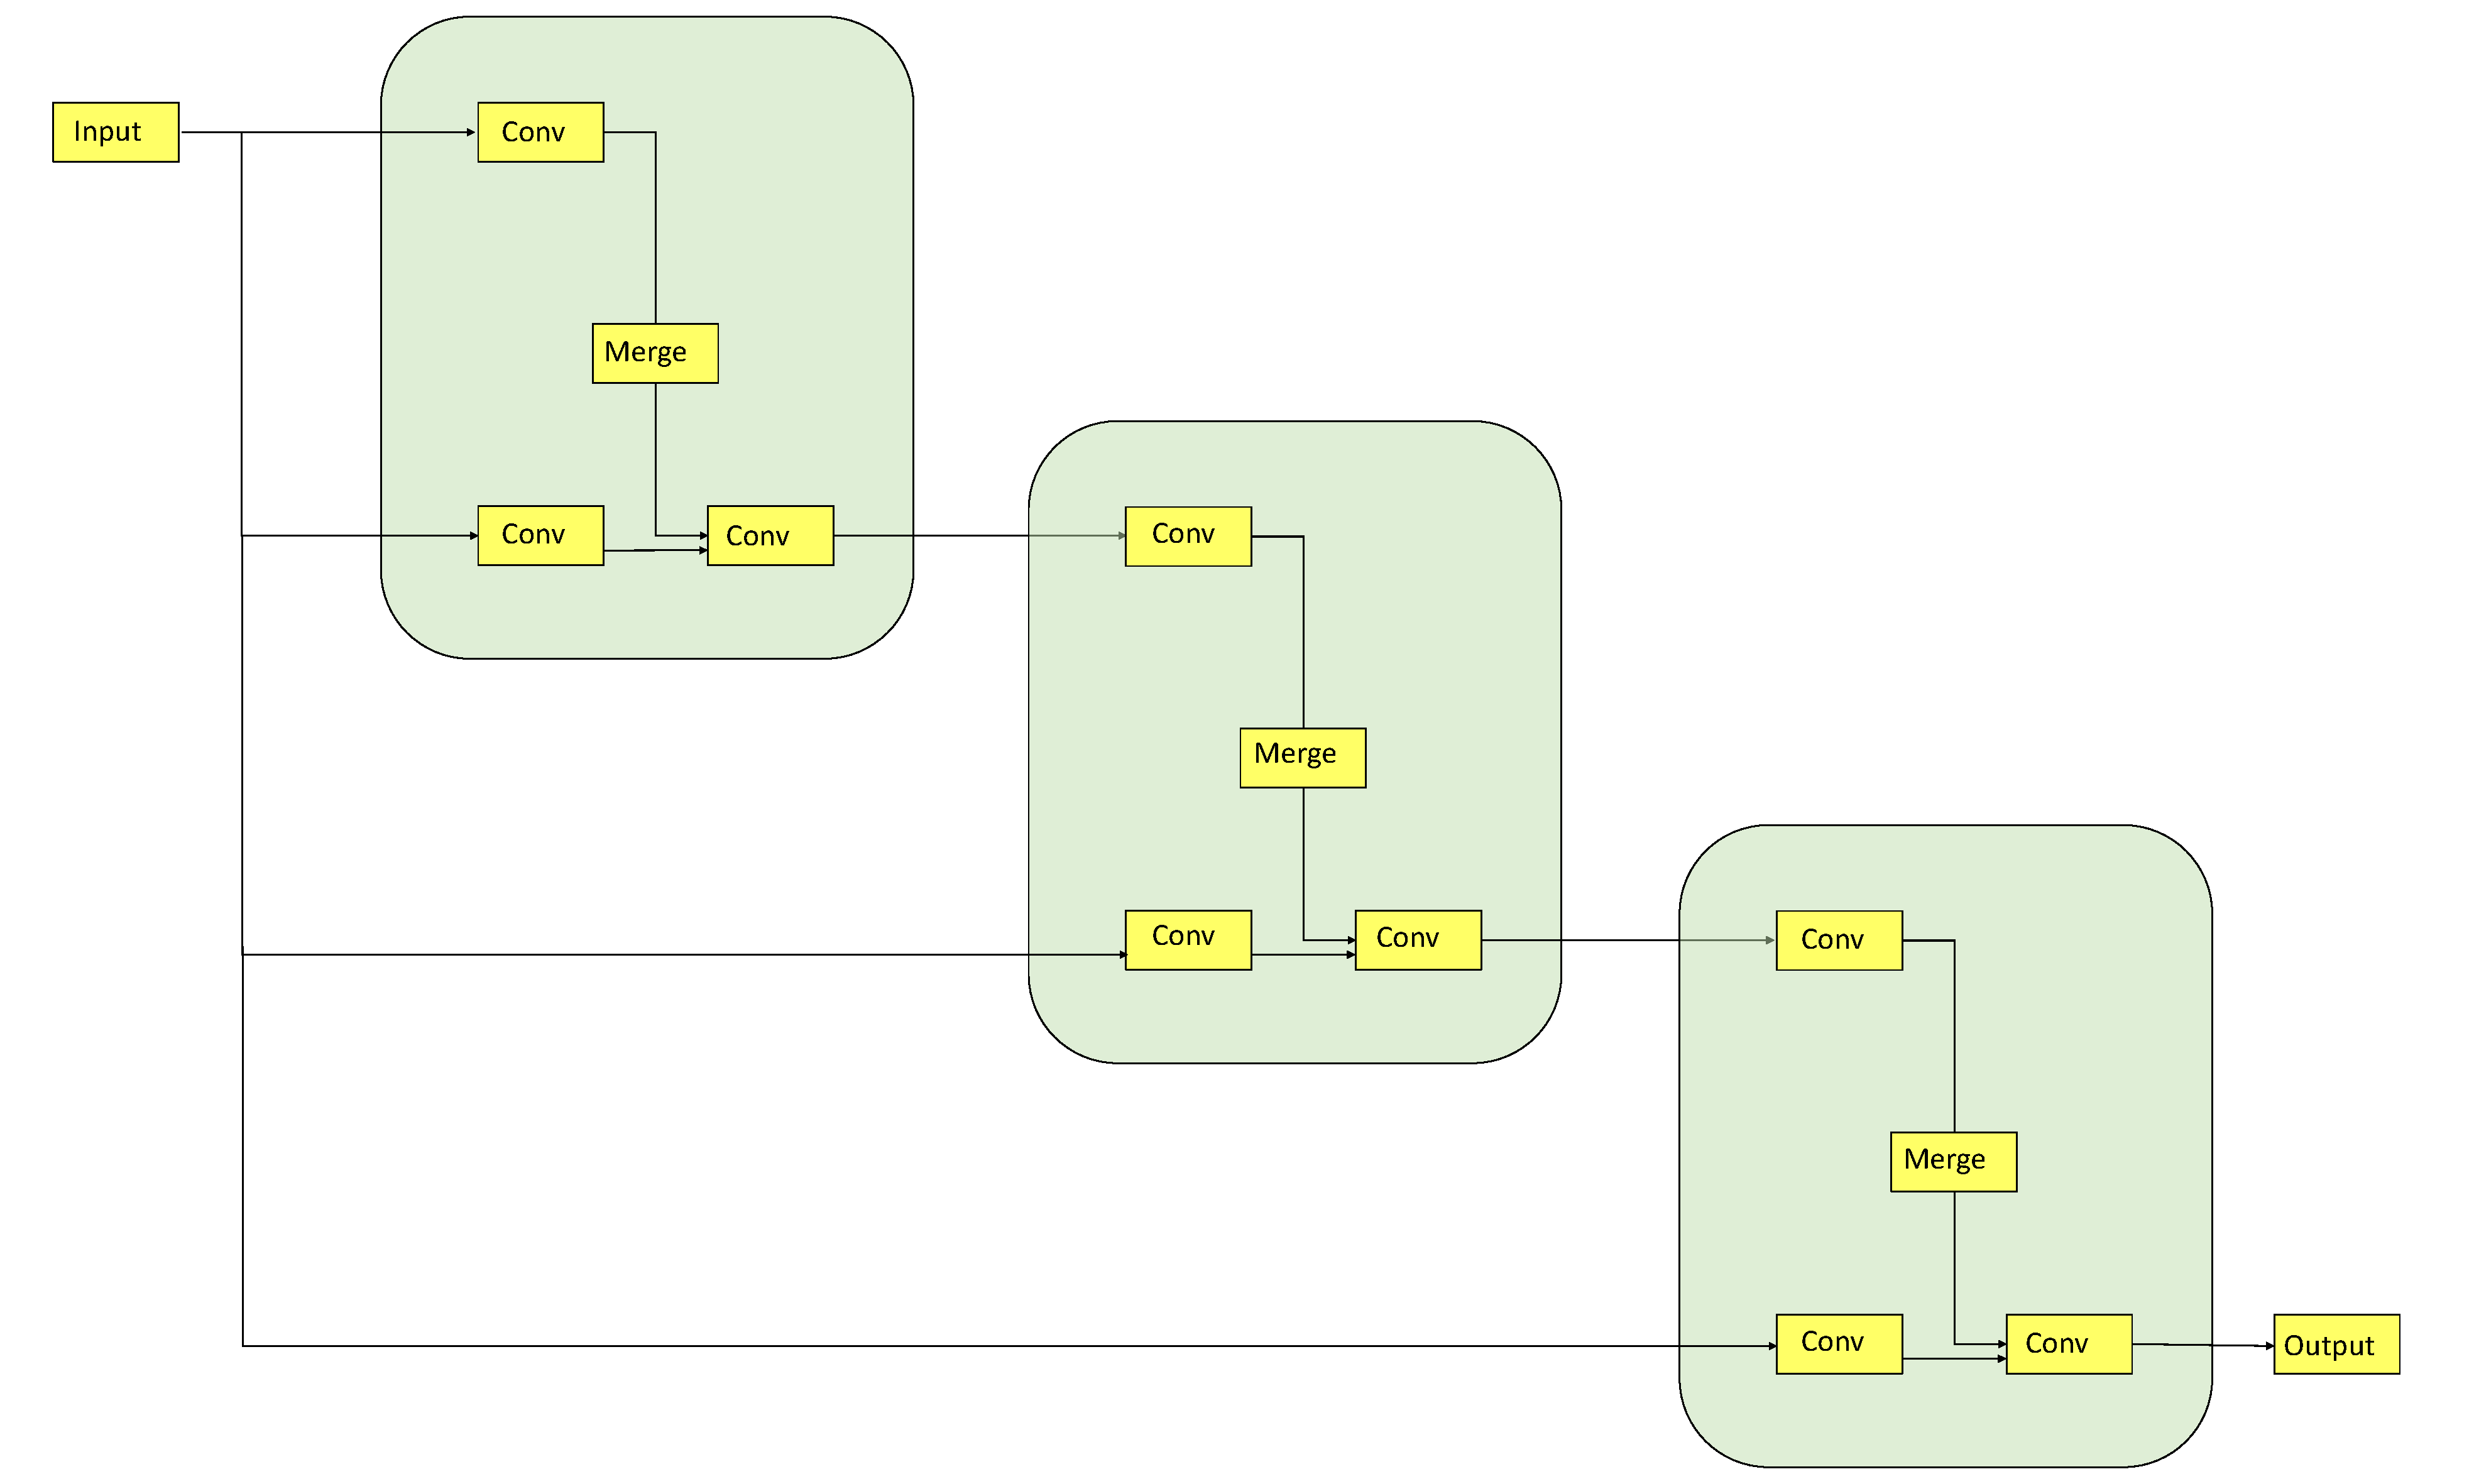
\includegraphics[width=0.5\textwidth]{./pic/design.pdf}
    \caption{Network Architecture of SRPeek.}
    \label{fig-system}
\end{figure}

\subsection{system design}


We implemented a holistic system for shoulder surfing, with the neural network as core, on a smartphone to verify the efficiency of our model. It iterates through the following steps: 
\begin{enumerate}

\item Input. Under guidance of the attacker, The smartphone will zoom in, take focus, and take 20 images with burst mode of the target screen. Note that the zoom in step is only for easier interaction and focusing, and to utilize the telephoto lenses and optical zoom, if avaliable, as digital zooming do not put in any extra data; On traditional phones with only digital zooming, the photo-taking will be with 1x zoom, and on phones with optical zooming, 5x to 10x zoom, depending on the optical zooming range. This way information on the images will be more compact and easier to comprehend by neural networks.

\item Alignment. The images are then aligned to mitigate the shifts between frames caused by hand tremor or movements from the lenses, as cameras with optical lenses will ocationally shift slightly across time due to the movements of its inner mechanism. Luckily, in our scenario the target is a glowing screen whose edges are easily distinguishable in most cases, and we use them as reference to align our images. The images are also spun to make the text horizontal in the process. The screen is cropped out and the rest of the image abandoned.

\item Adjustment. The lines of text(or stuff differing from the background color of the screen) will be carved out for processing, to reduce the workload of the network. The characters are normally around 10x10 pixels in the photos, and the carved segments will leave 2 pixels of padding on all sides to avoid mutilating the character; A certain amount of error is allowed, but if the size of the text is too small or too large, the neural network will not be able to extract features normally, so the images will be zoomed to the right size(and the zooming of step (1) will be adjusted accordingly).

\item Processing. As our network accepts only 9x9 patches, we will iteratively process all the overlapping 9x9 boxes among the input photo. For example, a 10x10 image will be four 9x9 patches, and a 11x11 image nine patches, etc(see fig.~\ref{fig-patches}. After carving a 9x9 patch at corresponding locations of each image, these patches are then processed by our multi-frame super resolution network, generating a single 36x36 image (4x upscaling). The input is RGB colored, while the output, as we are not interested in color, is black and white. When all patches are processed, their outputs are merged together. The overlapping pixels are thus processed: among all the outputs containing this pixel, we collect these values, remove outliers, and use their average as the result. In this way, we generate upscaled image segments of all the characters on the target screen, which are then inserted in one of the input images(roughly upscaled to encompass them, just for reference) and displayed to the attacker.

\begin{figure}
 \centering
    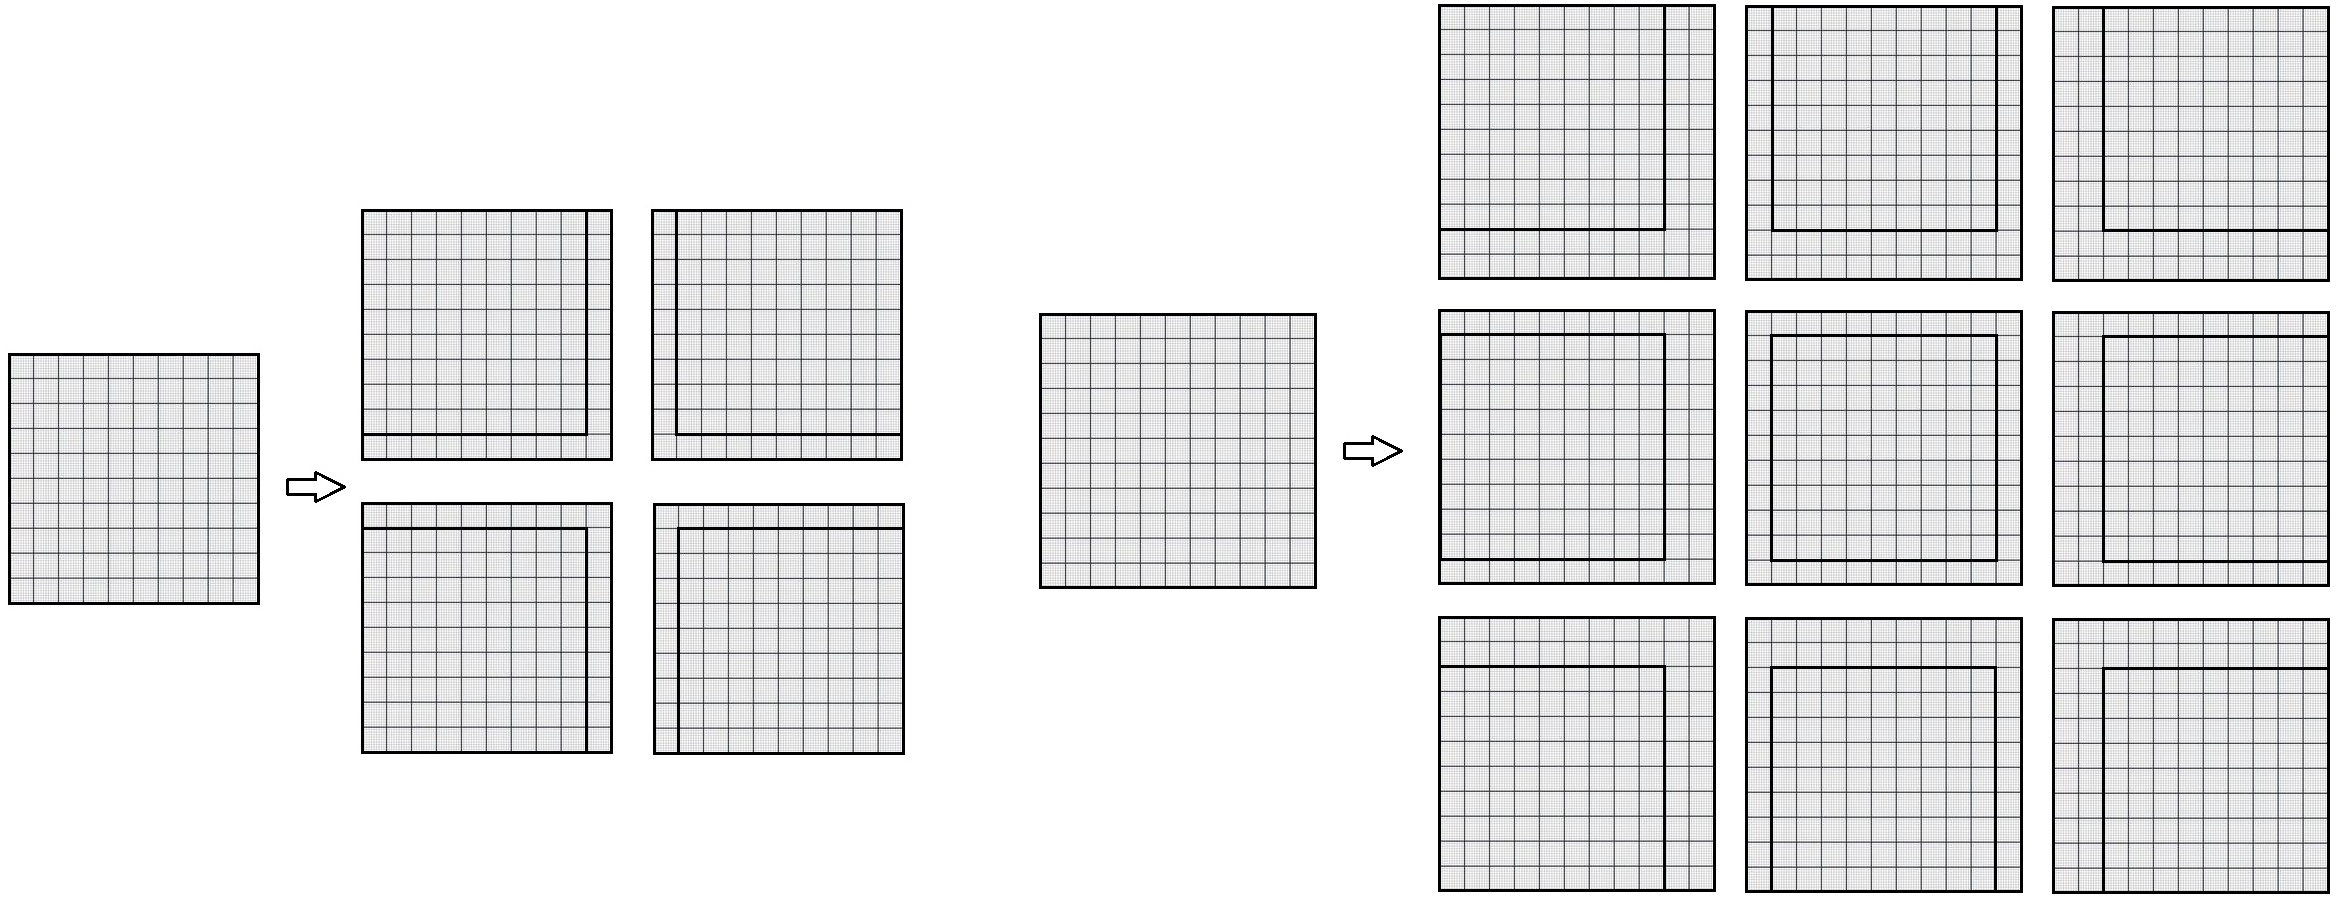
\includegraphics[width=0.5\textwidth]{./pic/patches.jpg}
    \caption{Illustration of overlapping patches the network process photos.}
    \label{fig-patches}
\end{figure}

\end{enumerate}

These steps are repeatedly executed to enable the attacker to monitor the victim at an interval of a few seconds. At critical times requiring continuous monitoring so as not to miss transient display, e.g. password entering, the system can simply lengthen the input phase across that period and process the data afterwards. The workflow of our system is shown in fig.~\ref{fig-workflow}.
\begin{figure}
 \centering
    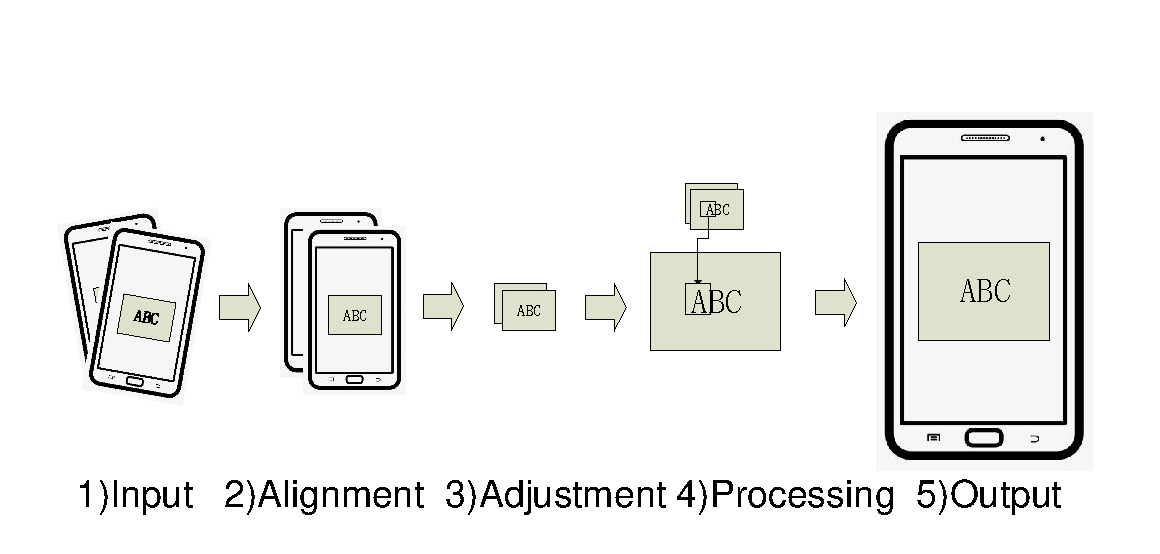
\includegraphics[width=0.5\textwidth]{./pic/workflow.pdf}
    \caption{Illustration of the workflow of our shoulder-surfing system.}
    \label{fig-workflow}
\end{figure}

